\documentclass[oribibl]{llncs}
 
\usepackage{amssymb} % AMS Fonts
\usepackage{amsmath} % AMSLaTeX
\usepackage{url}
\usepackage[pdftex]{graphicx}
\usepackage{slashbox}

% Compile only with pdfLaTeX
\usepackage[pdftex]{graphicx}

\newcommand{\ZZ}{{\mathbb{Z}}}
\newcommand{\QQ}{{\mathbb{Q}}}
\newcommand{\RR}{{\mathbb{R}}}
\newcommand{\CC}{{\mathbb{C}}}
\newcommand{\NN}{{\mathbb{N}}}
\renewcommand{\H}{{\mathcal{H}}}
\renewcommand{\L}{{\mathcal{L}}}
\newcommand{\F}{{\mathsf{F}}}
\newcommand{\bigO}{{\mathsf{O}}}
\newcommand{\R}{{\mathsf{R}}}
\newcommand{\Fp}{{\mathbb{F}_p}}
\newcommand{\Fq}{{\mathbb{F}_q}}
\newcommand{\Fqd}{{\mathbb{F}_{q^d}}}
\newcommand{\Fqe}{{\mathbb{F}_{q^e}}}
\newcommand{\Fz}{{\F[z]}}
\newcommand{\Fzf}{{\Fz /(f)}}
\newcommand{\Fzfe}{{\Fz /(f^e)}}
\newcommand{\Rn}{{\R^{n \times 1}}}
\newcommand{\Rnn}{{\R^{n \times n}}}
\newcommand{\Fden}{{\F^{den \times 1}}}
\newcommand{\Fdenden}{{\F^{den \times den}}}
\newcommand{\ZZp}{{\ZZ_p}}
\newcommand{\ZZpe}{{\ZZ_{p^e}}}
\newcommand{\nxn}{{n\times n}}
\newcommand{\calI}{{\mathcal I}}

\newcommand{\FD}{{\F[\partial;\sigma,\delta]}}
\newcommand{\D}{{\partial}}
\newcommand{\shift}{{\mathcal{S}}}
\newcommand{\diff}{{\lower3pt\hbox{\large$'$}}}
\renewcommand{\k}{{\mathsf{k}}}
\newcommand{\lclm}{{\mbox{\upshape lclm}}}
\newcommand{\lcrm}{{\mbox{\upshape lcrm}}}
\newcommand{\gcld}{{\mbox{\upshape gcld}}}
\newcommand{\gcrd}{{\mbox{\upshape GCRD}}}



\newcommand{\smallskipback}{\vspace{-\smallskipamount}}
\newcommand{\medskipback}{\vspace{-\medskipamount}}
\newcommand{\bigskipback}{\vspace{-\bigskipamount}}



%\reversemarginpar
\makeatletter
\@twosidefalse
\makeatother
%\renewcommand*{\marginfont}{\color{red}\bf}
%\newcommand{\TODO}[1]{\marginnote[#1]{}}

\bibliographystyle{alpha}

\begin{document}

\title{\textsc{CREST-Z3} - Automated Test Generation Capable of Nonlinear Constraints\\[12pt]
Project for CS846}

\author{X. Lan, M. Wexler, A. Heinle}

\institute{University of Waterloo, David R. Cheriton School of Computer Science}

\maketitle

\begin{abstract}
  In this project, we will explore \textsc{CREST-Z3} \cite{CRESTZ3}, an automated test case generator for C-programs. It is an extension of the tool \textsc{CREST} \cite{CREST} capable of solving non-linear constraints in the process of generating tests. We will discuss its capabilities, and the practical and theoretical limitations of this tool.
\end{abstract}

%%%%%%%%%%%%%%%%%%%%%%%%%%%%%%%%%%%%%%%%%%%%%%%%%%

\section{Introduction}

In the beginning of the course, there was a presentation given on the
paper \cite{godefroid2005dart}. The authors of this paper presented an
automated way of generating test sets for given programs written in
the programming language \textsc{C}. The main principle of that tool
appears in the literature as \textbf{Concolic Testing} (this terminology appeared
for the first time in the paper \cite{sen2005cute}).

Informally speaking, concolic testing refers to the concrete
execution of a program, given either random or specifically chosen
values for the variables. During this execution, one collects symbolic
conditions on the variables in order to reach code lines in which a branch occurs
(e.g. induced by an \texttt{if}-statement). Those conditions are fed
to a theorem prover, in order to solve for possible variable values to
enter each branch. With that, people are trying to generate test sets
that satisfy the best coverage of the code -- in terms of nodes in the
control flow graph -- as possible.

\textsc{CREST}, in its original version, used a theorem prover called
\textsc{YICES} (\cite{dutertre2006yices}) for the part of solving
conditions to enter a branch. It is a powerful tool, yet it has a
significant weakness: it can only deal with linear equations. This is
a strong restriction, since, for example, an equation like
$$x^2 = 14 \mod 47$$
for $x \in \ZZ$ could not be resolved.
Also in other concolic testing tools like \textsc{CUTE}
(\cite{sen2005cute}), \textsc{DART},
\textsc{EXE} (\cite{cadar2008exe}) and \textsc{PathCrawler}
(\cite{williams2005pathcrawler}), only linear equations are solvable.

This is the case for a good reason, as we will see in section \ref{sctn:Z3} where we discuss computational limitations we have considering nonlinear equations.

Nevertheless, for the nonlinear case, in the project \textsc{CREST-Z3}, the theorem prover was replaced
by \textsc{Microsoft'}s solution \textsc{Z3}
(\cite{de2008z3}), which can handle a broader range of equation types,
including nonlinear ones. \textsc{CREST-Z3}, its architecture and
its practicality will be the subject of this paper.

The paper is organized as follows: Section \ref{sctn:CRESTZ3} is
dedicated to \textsc{CREST}(-\textsc{Z3}). We will see how one can use
this tool, specifications of its architecture, and some limitations
that we found.

In section \ref{sctn:Z3}, we will examine those limitations a little
bit closer from a theoretical point of view. The limitations we will address are not just holding for this particular implementation, but are valid for any implementation that would try to do solving nonlinear constraints. A general overview of
\textsc{Z3} will also be provided.

Section \ref{sctn:Experiments} contains experiments we have done with
\textsc{CREST-Z3}. Furthermore, we are presenting types of \textsc{C/++}-projects
where nonlinear equations do play a role in the branching conditions
of the code. We will discuss how useful the extension \textsc{CREST-Z3} is in practical examples, and what extensions would be useful for the future.

Section \ref{sctn:Imrovements} discusses some improvements we made to CREST to allow for higher efficiency
and better user experience.

The last section draws a conclusion of our work.

All test files and program code we describe in this report can be found in our \textsc{GitHub} repository \url{https://github.com/wexlermi/dartnl}.

%%%%%%%%%%%%%%%%%%%%%%%%%%%%%%%%%%%%%%%%%%%%%%%%%%

\section{\textsc{CREST}(-\textsc{Z3})}
\label{sctn:CRESTZ3}

For notational convenience, we will from now on refer to
\textsc{CREST-Z3} as \textsc{CREST}. Most of the description of the
use of \textsc{CREST-Z3} can also be applied to the original
\textsc{CREST} project.

\subsection{How to use \textsc{CREST}}
We will start by presenting how one can use \textsc{CREST} to find
inputs in order to obtain reasonable code coverage.

One has to manually instrument code prior of running \textsc{CREST}.

Let us study how this is done using the following example:

\begin{example}
\label{ex:codeForDemo}
\begin{verbatim}

[1]   #include <crest.h>
[2]   #include <stdio.h>
[3]  
[4]   int main(int argc, char *argv[])
[5]   {
[6]     int w;
[7]     int x;
[8]     int y;
[9]     int z;
[10]    CREST_int(x);
[11]    CREST_int(y);
[12]    CREST_int(z);
[13]    CREST_int(w);
[14]    if (x*y + z == 0){
[15]      w = x*y*z;
[16]      if (w == z + x*y-1){
[17]        printf("GOAL %d %d %d %d\n", x, y, z, w);
[18]        return 1;
[19]      }
[20]    }	
[21]    return 0;
[22]  }
\end{verbatim}
\end{example}

The main steps are:
\begin{enumerate}
  \item Including the \texttt{crest.h} header file of the
    \textsc{CREST} project. (Line 1)
   \item For all variables that appear in branching nodes of the code
     (in this case the variables $x,y,z$ and $w$), one has to instruct
     \textsc{CREST} to collect symbolic conditions with respect to
     those variables during the
     execution. (Lines 10-13)
   \item OPTIONAL: Add a
     \texttt{printf} to every line inside conditional branch that
     outputs the variable values (Line 17). Then, during the execution of
     \textsc{CREST}, whenever a solution is found that enters the
     desired line of code (in this case line 18), an output is
     provided stating the calculated values for the variables.
\end{enumerate}

\begin{remark}
  This example already contains nonlinear constraints inside the
  \texttt{if}-statements and therefore serves as an example of how
  \textsc{CREST-Z3} extends the functionality of the classical \textsc{CREST}.
\end{remark}

\begin{remark}
  \label{rmrk:DataTypes}
  The datatypes \textsc{CREST} can handle in the current status of the
  project are: (unsigned) characters, (unsigned) integers, (unsigned) shorts.
\end{remark}

Then, after compiling the \textsc{CREST} project according to the
instructions, one runs inside the \texttt{bin} folder of the project
the program \texttt{crestc} with the instructed file as input. This
will generate the control flow graph and will collect initial information
about the program. For this code analysis step, the developers of
\textsc{CREST} utilize a tool called \textsc{CIL} (\cite{necula2002cil}).

As a result, in the same folder as the instructed file, several other
files will appear, including the compiled version of the
program. Those files are provided by \textsc{CIL} and one can find the
control flow graph and general information about the branching inside
the program there. %TODO: Discuss the files?

After that, in order to obtain possible values for the observed
variables for maximal code coverage, one has to run the tool
\texttt{run\_crest} with the following inputs:
\begin{itemize}
  \item The executable file that was compiled by \texttt{crestc}
  \item A number of maximal iterations through the control flow graph
    we want to allow (i.e. a limitation to the paths we
    want to consider. Otherwise the program might run too long)
  \item A strategy \textsc{CREST} should use to traverse the control
    flow graph. Possible options here are in the set
\begin{center}
$\{$\texttt{dfs}, \texttt{cfg}, \texttt{random},
    \texttt{uniform\_random}, \texttt{random\_input}, 
    \texttt{cfg\_baseline}, \texttt{hybrid}$\}$
\end{center}
\end{itemize}
For details on the respective search strategies consider
\cite{CREST}.

An example of this would be:
\begin{verbatim}
$ ../bin/run_crest ./hello 10 -dfs
\end{verbatim}

Consequently, in the same folder some new files do appear. One class of
files have a name of the form \texttt{input}${}^*$, where one can find possible input
values for the variables even if one has not added a \texttt{printf} line as in the
code above (Line 17). Another file is called \texttt{coverage} and contains the
nodes in the control flow graph indicated by numbers that are
covered. Additionally, one can find a file called
\texttt{szd\_execution}, where the intermediate symbolic formulas that
appeared during the execution of \texttt{run\_crest} can be found.

\begin{remark}
  The \texttt{input} files are only added by default in
  \textsc{CREST-Z3}, but not in the original \textsc{CREST}. In order
  to instrument \textsc{CREST} to do the same, one can follow the
  instructions given here: \url{https://code.google.com/p/crest/wiki/FAQ}.
\end{remark}

For the code given in Example \ref{ex:codeForDemo}, one of the \texttt{input}-files has
the following content:
\begin{verbatim}
-1
1
1
1409925863
\end{verbatim}

Thus $x :=-1, y:=1, z:=1$ and $ w:=1409925863$ would be possible
inputs to reach the code lines 17 and 18.

\begin{remark}
That $w$ has such a large
value is due to the fact that it does not matter what we put for $w$
as input, as it is redefined in line 15 dependent on $x,y$ and
$z$. Therefore, it did not play a role in any further symbolic
evaluation and the standard test value that is chosen randomly for the
first run is kept.
\end{remark}

\subsection{Limitations of \textsc{CREST} and Possible Workarounds}

We have created several small test cases to check what CREST can and
what it cannot -- or just partially -- do. In this section, we will only discuss
limitations that are independent from the solving technique used. The
theoretical and practical limitations of the solving routine is the subject of section \ref{sctn:Z3}.

\subsubsection{Constraints in handling the unary negative operator.}
During the course of our evaluation of CREST, we discovered that it is unable to handle the negative unary operator. For instance, the following code sample was unable to be solved by CREST:

\begin{example}
\begin{verbatim}

if ( x*x*x == -8){
    printf("GOAL %d\n", x);
    return 1;
}
\end{verbatim}
\end{example}

Surprisingly, a slight alternation of the code by replacing \texttt{x*x*x == -8} by \texttt{x*x*x+8==0} makes it possible to be solved. We suspect that there might be some bug in the generation of the formula, as we checked by hand if \textsc{Z3} is able to solve this formula and encountered -- not surprisingly considering the reputation of \textsc{Z3} -- a positive answer.
\subsubsection{Interprocedural Analysis Possible... Or Not?}

We discovered a reasonable flaw concerning interprocedural analysis.

Consider Example \ref{ex:codeForDemo} again, and assume we replace
line 14 by
\begin{verbatim}
if (f(x,y,z))
\end{verbatim}
where \texttt{f} is the following function:
\begin{verbatim}
f(int x, int y, int z){return x*y+z==0;}
\end{verbatim}

Using this instruction, \textsc{CREST} fails to produce possible
outputs to enter the branches induced by the modified \texttt{if}
statement.

However, let us replace line 14 is instead by

\begin{verbatim}
if (f_2(x,y,z)==0)
\end{verbatim}

where \texttt{f\_2} is the function
\begin{verbatim}
f_2(int x, int y, int z){return x*y+z;}
\end{verbatim}

Then everything works well and \textsc{CREST} is able to state and
solve the necessary equations to branch into the body of that \texttt{if}-statement.

But what went wrong? Studying the file \texttt{szd\_execution}, it
appears that it failed to produce the equations that need to be
solved. We suspect that this is due to the fact that during the
analysis process, \textsc{CREST} is not able to set conditions under
which conditions the boolean expression \texttt{x*y+z == 0} itself makes the
\texttt{if} statement evaluate to be true. If it is directly inside
the \texttt{if}-statement, it is clear to \textsc{CREST} how to
evaluate it. But in the case of \texttt{f}, it fails to reason that
\texttt{f} evaluates to
\texttt{1}, the \textsc{C} equivalence to \texttt{true}, exactly when \texttt{x*y+z == 0}.
This can be seen as an issue of the analysis process, and we will post
it right after this project is handed in.

\subsubsection{Double resp. Float Variables.}
\label{sbsbsctn:dblrespfloat}

We mentioned above (Remark \ref{rmrk:DataTypes}) the data types supported by \textsc{CREST}. What is
missing are datatypes like \texttt{float} or \texttt{double}.

In fact, as we will see in Section \ref{sctn:Experiments}, for a large set
of implementations where nonlinear equations play a role inside \texttt{if}
statements have floating point variables that determine the
evaluation.

For the original \textsc{CREST}, there exists a patch to extend its
functionality to be able to also handle floating point variables
(\url{https://code.google.com/p/crest/}, Issue \#15). Unfortunately, that
patch cannot analogously be applied to
\textsc{CREST-Z3}. We discovered that in order to obtain this functionality, we
would need to refactor large parts of the core of \textsc{CREST-Z3},
and this would go above and beyond the scope of our project.

\subsubsection{Arrays.}

Even though both \textsc{Z3} as well as \textsc{YICES} are capable of
handling array types, \textsc{CREST} does not support that as an
observable type. This can be seen as a flaw, even though there is a
workaround to this: In the original \textsc{CREST} paper
(\cite{CREST}), the authors were testing their software on the open
source program \textsc{grep} with a very high coverage rate (60\% of
the estimated coverable branches).

In fact, one variable they were observing in the project was \texttt{keys}, which is in fact an array. In order to
instrument \textsc{CREST} to do that, they put every entry of the
array into the scope of \textsc{CREST} in the following way:

\begin{verbatim}
[...]
keys = argv[optind++];
  keycc = strlen(keys);
  for(iii=0; iii<keycc;iii++){
    CREST_char(tmp1);
    keys[iii]=tmp1;
  }
  printf("%s\n",keys);
[...]
\end{verbatim}

This means that \textsc{CREST} adds, in every iteration of the
\texttt{for}-loop, \texttt{tmp1} as a new variable. From that moment on, it
knows that keys at certain position store an observed value and then
it can start performing evaluations based on that.

\subsubsection{No Automatic Instrumentation.}

For \textsc{CREST}, we need to manually instrument code in order to
clarify which variables it should observe. Depending on the size of
the project, this can be a very time-consuming task.  Furthermore, it requires
the program to be executable to work, i.e. one cannot utilize it for
pure in-between test generation for units, but either has to run it after
the project has reached the executable state, or one has to write in-between executable routines for the units. Both solutions are not optimal in general.

To solve this issue, we have written a script that automates this instrumentation process. It can be found in the \textsc{GitHub} repository of our project (\texttt{src/crest\_instrument.py}).


%Here: Software architecture of CREST ? (See Xiaoye's question)

%%%%%%%%%%%%%%%%%%%%%%%%%%%%%%%%%%%%%%%%%%%%%%%%%%


\section{\textsc{Z3} And the Problem of Solving Nonlinear Equations}
\label{sctn:Z3}

This section is dedicated especially to \textsc{Z3} and some theory
around solving nonlinear equations.

\subsection{Introduction to Z3}
The tool \textsc{Z3} \cite{de2008z3}  was developed by researchers from \textsc{Microsoft} to decide -- if
possible -- ``Satisfiability Modulo Theories'' (abbreviated SMT)
problems. These problems are given in first order logic and can be
seen as an extension to the satisfiability problem in predicate logic
(SAT), by introducing datatypes like numbers and their respective
operations. A standard to represent those formulas in an automatically
readable form was developed in the \textsc{SMT-LIB} project  \cite{barrett2010smt}.
The developers of \textsc{Z3} are using this standard as their
internal representation.

We will refrain from providing a detailed description of SMT problems
and their representation, as this would exceed the scope of this
report. But the following example will present the basic structure of
those problems:

\begin{example}
  Given the variables $x,y,z$, which we consider to
  be integer numbers, an SMT solver could answer the question of whether or not
  a solution for $x,y$ and $z$ exists, given the following
  constraints:
  \begin{enumerate}
    \item $x \neq y$
    \item $xy+x^2y=z$
    \item $|z|<10$.
  \end{enumerate}
  The solver would either state that it cannot solve this problem, or
  that no solution exists (provable), or it would provide values for
  $x,y$ and $z$ that satisfy the given conditions.
\end{example}

\textsc{Z3} can be included as a library to \textsc{C}/\textsc{++} source code, and one
can call the theorem prover from there. This is very handy, as one does
not have to parse any input to a tool and parse the output back, but instead can
just can call the respective functions inside his own functions.

The source code of \textsc{Z3} was recently (September 2012) published
by Microsoft (\url{http://z3.codeplex.com/}), so we could examine the
techniques the developers used to handle the nonlinear equations we
are looking for inside their code. We will go into more detail on that
after we discuss some theory behind nonlinear equations.

\subsection{Theoretical Limitations}

There are some theoretical limitations given considering the problem
of solving nonlinear equations.

We are given the following scenario: consider integer variables $x_1, \ldots,
x_n, n \in \NN$, and a boolean expression inside an if statement that
evaluates to true if and only if a polynomial given in those variables
is zero for some choice of $x_1, \ldots, x_n$. Finding a solution for
the $x_i$ is the so-called "Hilbert's tenth problem"
\cite{davis1984hilbert}, which was proven to be undecidable
\cite{matiyasevich1970enumerable}.

Despite the intractability of this problem, one can always try to find solutions and cancel the
computations after a certain amount of time.

Given a set of polynomial equations, the status quo to find solutions
is to first calculate the Gr\"obner basis of this system (originated by B. Buchberger in his PhD Thesis, consider e.g. in \cite{buchberger1970algorithmisches}). This can be seen as a
simplification of the system, which leads in the case of the existence
of only finitely many solutions directly to the solutions. Inside the
source code of \textsc{Z3}, we could also find an implementation of an
algorithm to calculate those bases.

But there is one problem to this approach: calculating a Gr\"obner
basis has double exponential complexity, independent of the choice
of the algorithm chosen to compute it (\cite{mayr1982complexity}). Therefore,
computations can take a long time, and the output may be quite simple, but is still hard to utilize it for finding the solutions. The next subsection will provide an example to illustrate
this fact.

Finding solutions to nonlinear equations is also heavily studied in current
research. Almost every computer algebra system provides a
functionality to solve systems of equations, but there are still
plenty of examples where those solvers do fail. Thus, one is also
limited by the possibilities current research provides.

\subsection{Practically Hard Problems}

In order to illustrate where one reaches those limitations, we
considered the following code:

\begin{verbatim}
int main(int argc, char *argv[]){
  int w;
  int x;
  int y;
  int z;
  if (x*x*y*y*y*z*z == 2700){
    if (x*x*y*w + y*y*w*w == 525){
      if ( x * y*w+y*y*y*w*w==1365){
        printf("GOAL %d %d %d %d\n", x, y, z, w);
          return 1;
        }
     }
  }
  return 0;
}
\end{verbatim}

In order to cover all branches, one could use as input $(x,y,z,w) :=
(2,3,5,7)$. \textsc{Z3} is not able to solve it. We stopped the
calculation after a couple of hours.

Let us examine the reason why it fails. \textsc{Z3} will try to compute
a Gr\"obner basis of the ideal generated by
\begin{eqnarray*}
  x^2y^3z^2 - 2700, \quad x^2yw + y^2w^2 - 525, \quad xyw + y^3w^2,
\end{eqnarray*}
and based on that result, it will try to solve the equation. As said,
solving for integer values is, in general, undecidable.

Let us look at the Gr\"obner basis for this system, which we
calculated using the computer algebra system \textsc{Singular}
\cite{Singular:2012}. The output is a polynomial system that fits into
a file of the size of 283KB. We will give a short snapshot of one
element in the output for the sake of visualization:

\begin{verbatim}
6755988021120000yw31-165994625678918400000yw30
+1737133233041462256000000yw29
-10103309530871289445440000000yw28
+35744012480436414061798800000000yw27
-79140476520758021570218836000000000yw26
+108725930332567845122270489310000000000yw25
-88760995051809423012610038134400000000000yw24
+39085314130645312603256453079810000000000000yw23
-7116024938996671115986413518424570000000000000yw22
+[...]
\end{verbatim}

\textsc{Singular} is specialized in performing those computations, and
it took several minutes to compute this Gr\"obner basis. There are
several factors that play a role how fast an algorithm computes this
Gr\"obner basis. One of them is how ``smart'' it is implemented. This
computation can take either minutes or hours, depending on the implementation.

Of course, one can also try to solve those equations directly using \textsc{Singular} or other 
state-of-the-art computer algebra systems. We observed that those will
not provide the easy solution that we know about this system.

The computer algebra system \textsc{Maple} (\cite{Maple}) e.g. outputs the following:
\begin{verbatim}
{w = w,
x = RootOf(13*w*_Z^6-5*w*_Z^5+13*w^2*_Z^3+(-5*w^2+20475*w)
    *_Z^2-5250*w*_Z-1378125+17745*w^2),
y = -(13*RootOf(13*w*_Z^6-5*w*_Z^5+13*w^2*_Z^3
    +(-5*w^2+20475*w)*_Z^2-5250*w*_Z-1378125+17745*w^2)^2*w[...],
z = 338*RootOf(-15138703125*w^6+61992127968750*w^5
    -12932841796875*w^4-4814544287109375*w^3[...]}
\end{verbatim}

This means that \textsc{Maple} recognizes that the value of $w$ can be
chosen arbitrarily and that the solution solely depends on the values
of $x,y$ and $z$. Furthermore, the solution of \textsc{Maple}
depends on algebraic extensions of the ground field (usually chosen to
be $\QQ$).

The computer algebra system \textsc{Sage} (\cite{sage}), which utilizes
\textsc{Maxima} (\cite{maxima}) for solving such equations, fails to
output any solution whatsoever.

The last computer algebra system that we tested for those purposes was
\textsc{Mathematica} \cite{wolfram1999mathematica}, in the context of
\textsc{Wolfram Alpha}\\ (\url{http://www.wolframalpha.com}). It found
several solutions, but not ones with integer values. One solution was,
for example:
\begin{verbatim}
w<-(25 sqrt(21))/13 and 
x = Root[13 #1^6 w-5 #1^5 w+13 #1^3 w^2+#1^2 (20475 w-5 w^2)-5250 #1
    w+17745 w^2-1378125&, 1]
and y = 1/2 (sqrt((x^4+2100)/w^2)-x^2/w)
and z = -30 sqrt(3) sqrt(1/(x^2 y^3))
\end{verbatim}

As a conclusion, one can see that deriving an integer solution using
external tools appears to be a very daunting task.

\subsection{Alternatives}

\textsc{Z3} is of course not the only \textsc{SMT}-solver that is
available, yet it belongs to the group of the most powerful
ones. Other tools that are capable of solving complex SMT's and that use the
same input as \textsc{Z3} are, for instance:
\begin{itemize}
  \item \textsc{Alt-Ergo} (\cite{bobotalt}) and
  \item \textsc{CVC4} (\cite{barrett2011cvc4}).
\end{itemize}

In the original \textsc{CREST} project, \textsc{YICES} (\cite{dutertre2006yices}) was used for
solving. It was not capable of nonlinear constraints, but accepted
input in the SMT-LIB standard. Therefore, replacing the SMT-solver in
the \textsc{CREST} project took only the instrumentation effort, which
can also be done similarly with the tools above. This would lead to an
interesting comparison between those tools regarding the branches in
code they are able to resolve.

Another approach that is, in our opinion, much more preferable would be
to utilize computer algebra systems such as the ones mentioned in the last subsection, 
which in general contain the implementations of the latest research techniques to solve equations
of all kinds. There is, of course, more instrumentation to be done in
order to get them to work within the \textsc{CREST} context, but the
extra effort will be paid back by lower calculation times plus more
robust results.

%%%%%%%%%%%%%%%%%%%%%%%%%%%%%%%%%%%%%%%%%%%%%%%%%%

\section{Experiments And Case Study}
\label{sctn:Experiments}

In this section, we will discuss some experiments on existing software
projects done with
\textsc{CREST}.

We will start by summarizing evaluations done in \cite{CREST} and
\cite{CRESTZ3}.

After that, we will discuss project types where evaluations of
nonlinear equations are likely to be found in \textsc{C/++} programs, and how common the use
of nonlinear equations within boolean expressions is.

We will conclude this section by evaluating CREST on a set of test cases we generated, and we will
examine some key metrics that give insight into the accuracy and performance of CREST.

\subsection{Summary of Former Evaluations}

The author of \cite{CREST} has tested the original program on three
different source codes:

\begin{itemize}
  \item \textsc{Vim} (\cite{oualline2001vi}), $\sim 150,000$locl
  \item \textsc{Grep} (\url{http://www.gnu.org/software/grep/}), $\sim
    15,000$loc
  \item \textsc{Replace} (\cite{harrold2010siemens}), $\sim 600$loc
\end{itemize}

He was able to cover over 90\% of \textsc{Replace} within some
minutes. Around 60\% of the branches in \textsc{Grep} were covered
within a couple of minutes, where one could partly make improvements
using different search strategies. For \textsc{Vim}, he only instructed \textsc{CREST} to analyze some modes of the editor, with a
sample input. Within 2-3 hours he was able to cover up to one third
of all branches that were reachable.

In the paper about \textsc{CREST-Z3} (\cite{CRESTZ3}), one can only
find simple proof of concepts that it extends the classical
\textsc{CREST}. A large test on real world programs has not been made.

\subsection{The Frequency of Nonlinear Equations Appear in Real World
  programs}

\subsubsection{Ad Real World Programs According to the Limitations.}
First, we were searching for \texttt{if}-statements in programs that
contain nonlinear expressions in the supported types. Our search was
not fruitful, and only brought up a few examples that contained the
desired property.

Considering the \textsc{CRYPTO++} library
(\url{http://www.cryptopp.com/}, a \textsc{C++} library containing all kinds of algorithms from the field of cryptography), we could only find a few, fairly
simple tests of the following format:

\begin{verbatim}
<<rsa.cpp>>
[...]
[168] Integer a = modn.Exponentiate(i, r);
[169] if (a == 1)
[170]     continue;
[...]
\end{verbatim}

Those examples are not very hard to solve.

Looking at the source code of the computer algebra systems \textsc{Singular} (\cite{Singular:2012})
and \textsc{GAP} (\cite{GAP4}), where we assumed to find examples,
revealed that there is no occurrence of boolean expressions consisting
of nonlinear expressions to be
found in the code.

Our conclusion is that nonlinear constraints with the standard
supported datatypes in \textsc{CREST} are very rare to be found in
real life \textsc{C} code.

\subsubsection{Ad Real World Programs outside the Limitations.}

If we assume that floating point numbers would also be supported, the
range of real world programs that contain boolean expression based on
nonlinear equations is much higher.

The first type of programs where those types of equations do appear
are coming from the field of computer graphics. In the technique called ``ray
tracing'' (\cite{glassner1989introduction}) for example, they are very common. The following code snippet serves as an example in what way one finds them there (taken from \url{http://www.codermind.com/articles/Raytracer-in-C++-Part-I-First-rays.html}):
\begin{verbatim}
[...]
[1] double B = r.dir * dist;
[2] double D = B*B - dist * dist + s.size * s.size; 
[3] if (D < 0.0f) 
[4]     return false; 
[5] double t0 = B - sqrt(D); 
[6] double t1 = B + sqrt(D);
[7] bool retvalue = false;  
[9] if ((t0 > 0.1f) && (t0 < t)) 
[...]
\end{verbatim}

In line 2, the variable \texttt{D} is calculated using a nonlinear polynomial
formula. In the next line it is checked whether the result is smaller
than zero or not.
This code snippet furthermore shows an inconvenience we would obtain
if we would allow floating point numbers, namely the square root use
in line 5 and 6 and the boolean expression based on it in line 9. There are publications on ways to define square root and other
floating point typical operations that extend \textsc{SMT-LIB},
e.g. \cite{rummer2010smt}, and the basic preliminaries are included in
the \textsc{SMT-LIB} version 2.0. Nonetheless, we could not find the
full support of the arithmetic in the solvers. If one would extend
\textsc{CREST-Z3} to also handle floating point numbers, this problem
should also be taken into consideration.

Another area where we found boolean expressions based on nonlinear equations in floating point numbers were algorithms coming from finance. There is an interesting collection of \textsc{C++} programs in \cite{odegaard2003financial}. The way they appear there mostly is in converging constraints and in early termination of a program if a certain formula is fulfilled. The same holds for algorithms coming from numerics; consider for example the project \textsc{LAMMPS} (Mollecular Dynamics Simulator, \cite{plimpton2007lammps}).

Summa summarum one can say that considering nonlinear constraints, in practice it is only reasonable to additionally consider them if also floating point numbers are supported. For the supported datatypes, one rarely finds code where those play a significant, non-trivial role.

\subsection{Some Empirical Experiments on the Solving Ability of \textsc{CREST-Z3}}
We evaluated CREST for both performance and accuracy. To measure performance, we measured the time it took for CREST to analyze a given program. To measure accuracy, we measured the following two variables: program depth, and branch coverage. Due to the fact that CREST cannot handle the unary minus operator, which is prevalent in most real-world programs, we had to create our own test set of programs to evaluate on CREST. We wrote a test-set generator \textsc{createTestFiles.py} that, given several parameters, creates a random C file containing a certain amount nested if-statements, each of which contain an equation, as part of a total system of equations. 

Here we present a sample C program that we generated, specified to have 3 variables, and a nested-depth of 2 :

\begin{verbatim}
#include <stdio.h>
int main() {
	int x0;
	int x1;
	int x2;
    if ( 9 * x0 * x0 + 4 * x2 * x2 + 8 * x0 * x1 == 500 ) {
        printf("Solved the if at depth 1.\n");
        if ( 9 * x0 * x1 + 8 * x2 * x2 + 6 * x1 * x2 == 728 ) {
            printf("Solved the if at depth 2.\n");
        }
        else {
        	printf("At the else at depth 2.\n");
        }
    }
    else {
        printf("At the else at depth 1.\n");
    }
}
\end{verbatim}

We were interested in exploring the effect on program timing and coverage caused by changing several independent variables. The independent variables we analyzed were number-of-variables, nested-depth, and search-type. By search-type, we mean the type of search that CREST uses to traverse the program's control-flow-graph. For testing purposes, this can be one of the following three: DFS, random, and hybrid.

During the course of our analysis, we realized that CREST would often take a long time to analyze programs of large depth or large number of variables. For this reason, in our test script, we decided to make CREST timeout when the analysis took longer than 40 seconds.

Using the aforementioned script, we generated a test-set of 75 C files, which consists of 3 unique C files for each tuple (number-variables, nested-depth), where number-variables and nested-depth range from 1 to 5. For the equations in each if-statement, we restricted the total degree for any individual monomial to be 2. Future analysis could change this variable, and see how the dependent variables change.



Table 1 represents the timings when running CREST on our test-set using DFS (depth-first-search) search-mode:

\begin{table}[htbp]
\caption{}
\begin{tabular}{|l|r|r|r|r|r|l|}
\hline
 & \multicolumn{1}{l|}{} & \multicolumn{1}{l|}{Num-variables} & \multicolumn{1}{l|}{} & \multicolumn{1}{l|}{} & \multicolumn{1}{l|}{} &  \\ \hline
 & \multicolumn{1}{l|}{} & 1 & 2 & 3 & 4 & \multicolumn{1}{r|}{5} \\ \hline
Nested-depth & 1 & 0.131 & 0.163 & 0.112 & 2.482 & \multicolumn{1}{r|}{1.19} \\ \hline
 & 2 & 0.129 & 0.147 & 26.738 & 26.751 & ---- \\ \hline
 & 3 & 0.111 & 0.133 & 6.354 & 27.138 & ---- \\ \hline
 & 4 & 0.124 & 0.135 & 27.068 & \multicolumn{1}{l|}{----} & \multicolumn{1}{r|}{26.789} \\ \hline
 & 5 & 0.167 & 0.244 & 1.393 & \multicolumn{1}{l|}{----} & ---- \\ \hline
\end{tabular}
\label{DFS timings (in seconds)}
\end{table}

\begin{figure}[!t]
\centering
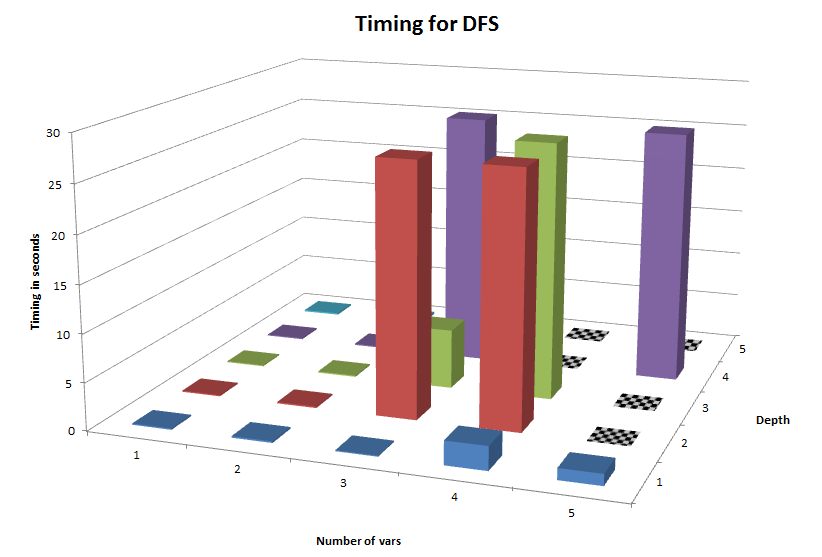
\includegraphics[width=13cm]{dfs_timings}
\caption{}
\label{figure:motivation}
\end{figure}

Figure 1 gives a graphical view of Table 1. The checkered squares of Figure 1 represent tests where the timing went past our threshold of 40 seconds. When we tested several of these programs by hand, we waited for an hour or so, and CREST still did not finish analyzing it. The results seem to confirm our guess that CREST runtime increases as the number of variables and the number of nested if-statements increase. We were a bit disconcerted to see that several of our test cases were unable to be solved by CREST in a feasible amount of time. Our previous discussion already mentioned some of the performance issues of non-linear equation solving.

\begin{table}[htbp]
\caption{DFS branch-coverage-ratio}
\begin{tabular}{|l|r|r|r|r|r|r|}
\hline
 & \multicolumn{1}{l|}{} & \multicolumn{1}{l|}{Num-vars} & \multicolumn{1}{l|}{} & \multicolumn{1}{l|}{} & \multicolumn{1}{l|}{} & \multicolumn{1}{l|}{} \\ \hline
 & \multicolumn{1}{l|}{} & 1 & 2 & 3 & 4 & 5 \\ \hline
Depth & 1 & 1 & 1 & 1 & 1 & 1 \\ \hline
 & 2 & 0.75 & 0.75 & 0.25 & 0.25 & 0 \\ \hline
 & 3 & 0.667 & 0.667 & 0.667 & 0.333 & 0 \\ \hline
 & 4 & 0.625 & 0.75 & 0.25 & 0 & 0 \\ \hline
 & 5 & 0.6 & 0.7 & 0.6 & 0 & 0 \\ \hline
\end{tabular}
\label{DFS branch-coverage-ratio}
\end{table}


\begin{figure}[!t]
\centering
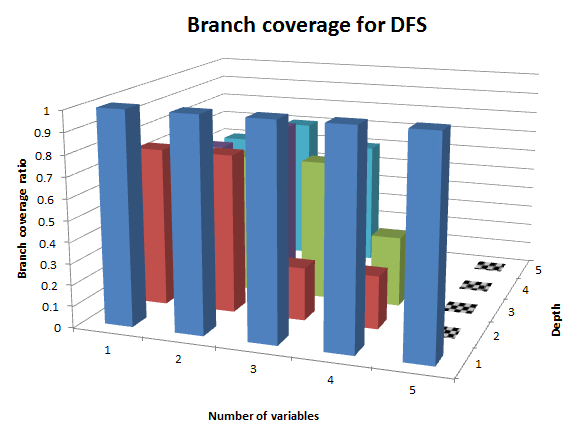
\includegraphics[width=13cm]{dfs_branch_coverage}
\caption{}
\label{figure:motivation}
\end{figure}

Figure 2/Table 2 show the results of measuring branch coverage for the DFS run-mode. By branch coverage, we mean the number of branches in the control-flow-graph that CREST was able to get to. Since every if-statement has a corresponding else-statement in our test set, the number of total branches for a given program is twice the depth. We found that as the number of variables in a program increased, the branch-coverage-ratio decreased, because it made it more difficult for Z3 to solve the constraints. Additionally, as we increase the program depth by one, the number of total branches increases by a factor of 2. This lowers the branch-coverage-ratio immensely.

\begin{table}[htbp]
\caption{Results for running CREST for depth = number-variables = 3}
\begin{tabular}{|l|r|r|r|}
\hline
 & \multicolumn{1}{l|}{DFS} & \multicolumn{1}{l|}{Random} & \multicolumn{1}{l|}{Hybrid} \\ \hline
Runtime (seconds) & 6.354 & 13.572 & 13.49 \\ \hline
Branch-coverage-ratio & 0.667 & 0.222 & 0.5 \\ \hline
\end{tabular}
\label{DFS timings (in seconds)}
\end{table}

Table 3 summarizes the performance and accuracy of CREST on the test-files corresponding to depth = number-variables = 3. We find that DFS gives the best performance and accuracy of the three run-modes, while random gives the worst results.

\section{Our Improvements to CREST}
\label{sctn:Improvements}
We accomplished several tasks that we believe will make CREST a more usable tool. We created a web interface for CREST, located at \url{http://dahu.in/crest.html}. At this web interface, one can submit a C file of his choosing, and examine the output that CREST would generate. We believe that this makes it much easier for one to test out CREST, without having to actually go to the trouble of downloading and installing it. From our own experience, the installation of CREST is quite a painful one, as the documentation on the CREST website does not cover many crucial steps that we discovered only through trial and error.

The second improvement that we made to CREST (as mentioned previously) is the development of a Python script that automatically instruments C code so it can work with CREST. CREST has the unfortunate property that all C files must explicitly declare their variables in a CREST format. Our script automatically instruments C code so this step is not necessary. In fact, our script recursively instruments all C files in a given directory, so an entire project can be instrumented for CREST very easily.

%%%%%%%%%%%%%%%%%%%%%%%%%%%%%%%%%%%%%%%%%%%%%%%%%%

\section{Conclusion and Future Work}
\label{sctn:Conclusion}

There are several conclusions we can draw in this report.

The first one is that \textsc{CREST(-Z3)} as a tool has to be made more robust. Some of the limitations we have found (like the one connected to interprocedural analysis), are flaws coming directly from the analysis process.

In order to really extend the functionality of \textsc{CREST} for real world programs, one also has to consider floating point numbers as possible data types, as for those nonlinear equations in boolean are more likely to appear. For the supported types, the original \textsc{CREST} suffices on our set of real world programs.

Concerning the question of which problem solver to use, we have seen that there are limitations from theory. Nevertheless, computer algebra systems contain the most recent algorithms coming from mathematicians all over the world. The solving part could be partially outsourced instead of using solvers implemented in \textsc{Z3} or other software projects. This would in our opinion increase the quality of those solvers in terms of equations they are able to solve.

A possible future task could be to deal with the constraints of \textsc{CREST(-Z3)}. Resolving them is not trivial. Furthermore, one could make the solving process more flexible, i.e. the solver replacable without any instrumentation, and possibly having several by hand at once.

Another future task is related to the question whether we are content with just node coverage on the control flow graph or not. \textsc{CREST-Z3} is performing only node coverage, and maybe it would be interesting to also perform some criteria like prime path coverage (see \cite{ammann2008introduction}). As with considering paths, we also gain more constraints on our variables, it might lead to an easier way to solve for those variables or prove the infeasibility. It would lead to a more flexible way of test generation that would be of interest for academia as well as for industry.

%Here: Extension to other programming languages? Or even Computer algebra systems?
%         Feasible for real world, as conditions do not get very complicated in general
%         Good for testing software that implements formulas or approximations.
%         Extending it to more general data-types?

%%%%%%%%%%%%%%%%%%%%%%%%%%%%%%%%%%%%%%%%%%%%%%%%%%

\bibliographystyle{plain}
\bibliography{report}

\end{document}
